\documentclass[11pt]{article}
\usepackage[utf8]{inputenc}
\usepackage[colorlinks=true, linkcolor=blue, urlcolor=cyan]{hyperref}
\usepackage{graphicx}
\usepackage[left=25mm, top=25mm, bottom=30mm, right=25mm]{geometry}

\renewcommand\thesubsection{\thesection(\alph{subsection})}
\renewcommand\thesubsubsection{\thesubsection(\roman{subsubsection})}

\title{COL334: Assignment 1}
\author{Sayam Sethi}
\date{August 2021}

\begin{document}

\maketitle

\tableofcontents

\section{Networking Tools}

\subsection{Local IP Address}
To obtain the \textit{IP address} of a device, running \texttt{ifconfig} gives the detailed information about the same.

\subsubsection{Router}
The following output is obtained on running the command when connected to Wi-Fi router:
\begin{center}
    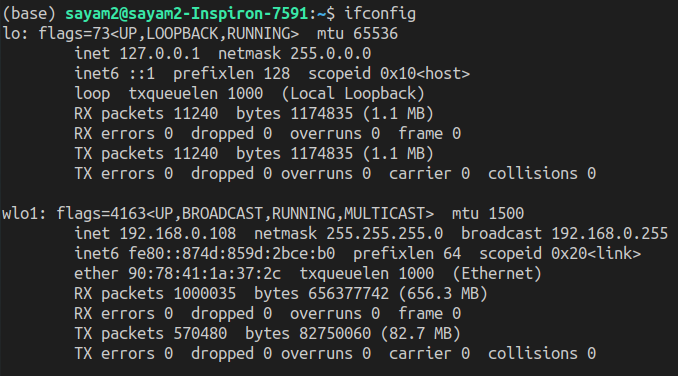
\includegraphics[width=0.5\linewidth]{figures/ifconfig_router.png}
\end{center}
The first entry in the output, i.e., \texttt{lo}, is the \textbf{loopback connection} which is used to connect to ports on the same device.\par
The second entry, \texttt{wlo1}, is the relevant one and it contains information about the \textbf{Wi-Fi connection}. The \textit{IP address} is the \texttt{inet} address: $192.168.0.108$.

\subsubsection{Mobile Hotspot}
On connecting to mobile hotspot, following is the output of \texttt{ifconfig}:
\begin{center}
    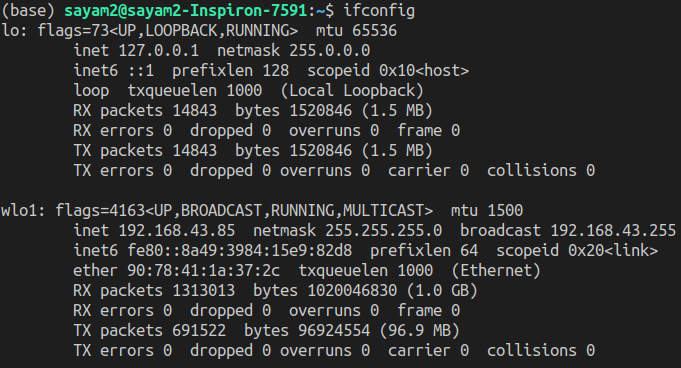
\includegraphics[width=0.5\linewidth]{figures/ifconfig_hotspot.png}
\end{center}
The \textit{IP address} which is the \texttt{inet} address now has changed to: $192.168.43.85$.


\subsection{IP Address of Different Servers}
To obtain the \textit{IP address} of servers, the \texttt{nslookup} command is used. This \textit{IP address} depends on the \textbf{DNS server} being used.

\subsubsection{\href{https://www.google.com}{Google}}
\begin{center}
    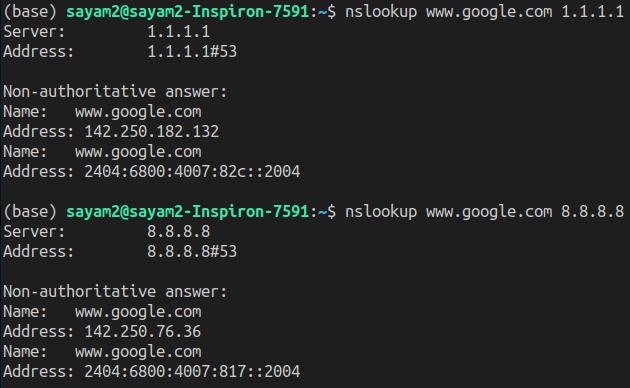
\includegraphics[width=0.5\linewidth]{figures/nslookup_google.png}
\end{center}
Using \textbf{Cloudfare 1.1.1.1 DNS} server gave the \textit{IP address} as $142.250.182.132$, while using \textbf{Google Public DNS} server resulted in an \textit{IP address} of $142.250.76.36$.

\subsubsection{\href{https://www.facebook.com}{Facebook}}
\begin{center}
    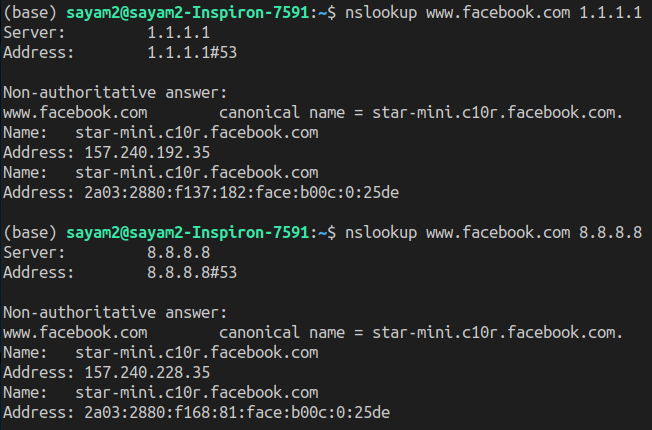
\includegraphics[width=0.5\linewidth]{figures/nslookup_facebook.png}
\end{center}
Using \textbf{Cloudfare 1.1.1.1 DNS} server gave the \textit{IP address} as $157.240.192.35$, while using \textbf{Google Public DNS} server resulted in an \textit{IP address} of $157.240.228.35$.


\subsection{Ping (Pong)}
To analyse the ping values, a script was written to \textbf{binary search} on different values of \textit{packet size} and \textit{TTL value}.\par
The size of the transmitted packet is always $28$ bytes larger than the size set using the \texttt{-s} command. This is the header data which has the same structure for all packets.

\subsubsection{Packet Size}

\paragraph{\href{https://www.iitd.ac.in}{IITD}} The maximum packet size that can be pinged is $29116\ (+28)$ bytes.
\paragraph{\href{https://www.google.com}{Google}} The maximum pingable packet size is only $68\ (+28)$ bytes.
\paragraph{\href{https://www.facebook.com}{Facebook}} The maximum packet size that is pinged is $1452\ (+28)$ bytes.

\subsubsection{Time To Live (TTL) Value}

\paragraph{\href{https://www.iitd.ac.in}{IITD}} The smallest TTL value achieved is $12$ hops.
\paragraph{\href{https://www.google.com}{Google}} The least number of hops taken to ping Google is $8$ hops.
\paragraph{\href{https://www.facebook.com}{Facebook}} Facebook is reached within atleast $10$ hops.





















\end{document}

